%================================================================
\appendix
% Additional calculations used to validate the codes, these 
% selected calculations can be listed with few comments. Can also 
% include listing of the code if you feel this is necessary
%================================================================
\section{Terrain data}\label{ap:terrain_data}
Information on the terrain data used in this project, downloaded from EarthExplorer.
\begin{table}[h]
    \centering
    \begin{tabular}{ccc}
        \hline
        Country & Coordinates & Filemane \\
        \hline
        China & $(36, 110)$ & \verb|n36_e110_1arc_v3.tif| \\
        Egypt & $(26, 29)$ & \verb|n26_e029_1arc_v3.tif| \\
        Japan & $(34, 135)$ & \verb|n34_e135_1arc_v3.tif| \\
        Nepal & $(27, 85)$ & \verb|n27_e085_1arc_v3.tif| \\
        Norway & $(59, 10)$ & \verb|n59_e010_1arc_v3.tif| \\
        \hline
    \end{tabular}
    \caption{Terrain data from different countries, files are located in the folder. The coordinates are with respect to the south west corner of the grid, given in latitude, longitude.}
    \label{tab:terrain_data}
\end{table}


\section{Bias-Variance Trade-Off}\label{ap:bias_var_eq}
The parameters $\mathbf{\beta}$ can be found by optimizing the cost function
\begin{equation*}
    C(\mathbf{X}, \mathbf{\beta}) = \frac{1}{n} \sum_{i=0}^{n-1} ( y_{i} - \Tilde{y}_{i} )^{2} = \mathbb{E} \big[ ( \mathbf{y} - \mathbf{\Tilde{y}} )^{2} \big] .
\end{equation*}
Assuming linearity, the expression can be written as 
\begin{equation*}
    \mathbb{E} \big[ ( \mathbf{y} - \mathbf{\Tilde{y}} )^{2} \big] = \mathbb{E} [ \mathbf{y}^{2} ] - 2 \mathbb{E} [ \mathbf{y} \mathbf{\Tilde{y}} ] + \mathbb{E} [ \mathbf{\Tilde{y}}^{2} ].
\end{equation*}
Looking at the first term
\begin{align*}
    \mathbb{E} [ \mathbf{y}^{2} ] &= \mathbb{E} [ ( f(\mathbf{x}) + \mathbf{\epsilon} )^{2} ] \\
    &= \mathbb{E} [ f(\mathbf{x})^{2} ] - 2 \mathbb{E} [ f(\mathbf{x}) \mathbf{\epsilon} ] + \mathbb{E} [ \mathbf{\epsilon}^{2} ] \\
    &= f(\mathbf{x})^{2} + \sigma^{2} ,
\end{align*}
where $f(\mathbf{x})$ and $\epsilon$ are independent of $\mathbf{y}$, and each other. The second term can be written as 
\begin{align*}
    \mathbb{E} [ \mathbf{y} \mathbf{\Tilde{y}} ] &= \mathbb{E} [ f(\mathbf{x} + \mathbf{\epsilon}) \mathbf{\Tilde{y}} ] \\
    &= \mathbb{E} [ f(\mathbf{x}) \mathbf{\Tilde{y}} ] + \mathbb{E} [ \epsilon \mathbf{\Tilde{y}} ] \\
    &=  f(\mathbf{x}) \mathbb{E} [ \mathbf{\Tilde{y}} ] & \text{since $\mathbb{E}[\mathbf{\epsilon}] = 0$} .
\end{align*}
The last term is the 2. moment, which can be written as 
\begin{align*}
    \mathbb{E} [ \mathbf{\Tilde{y}}^{2} ] &= \mathbb{V}[\mathbf{\Tilde{y}}] + (\mathbb{E} [ \mathbf{\Tilde{y}} ])^{2} 
\end{align*}
Combining all the terms, and rearranging gives us
\begin{align*}
    &\mathbb{E} [ \mathbf{y}^{2} ] - 2 \mathbb{E} [ \mathbf{y} \mathbf{\Tilde{y}} ] + \mathbb{E} [ \mathbf{\Tilde{y}}^{2} ] \\ 
    &= f(\mathbf{x})^{2} + \sigma^{2} - 2 f(\mathbf{x}) \mathbb{E} [ \mathbf{\Tilde{y}} ] + \mathbb{V}[\mathbf{\Tilde{y}}] + (\mathbb{E} [ \mathbf{\Tilde{y}} ])^{2} \\
    &= \mathbb{E} [ (\mathbf{y} - \mathbf{\Tilde{y}})^{2} ] + \mathbb{V}[\mathbf{\Tilde{y}}] + \sigma^{2} , 
\end{align*}
where 
\begin{align*}
    \mathbb{E} [ (\mathbf{y} - \mathbf{\Tilde{y}})^{2} ] = \text{Bias}[\mathbf{\Tilde{y}}]. 
\end{align*}

The bias-variance trade-off is a way to evaluate the how well the model is able to fit the test data. As seen in Figure \ref{fig:bias-variance}, when the polynomial degree is low, there is not much variance between the training data and the test data. However, the bias might be higher as it fails to predict the right complexity of the data. As the polynomial degree of the input increases, the variance increases. The bias decreases until the sufficient model complexity is reached. This is where the model is able to fit the training data, without overfitting, and also make good predictions on test data. 


\section{Additional analysis}\label{ap:additional_analysis}
The following figures show results from OLS regression, when feature scaling was applied.
\begin{figure}
    \centering
    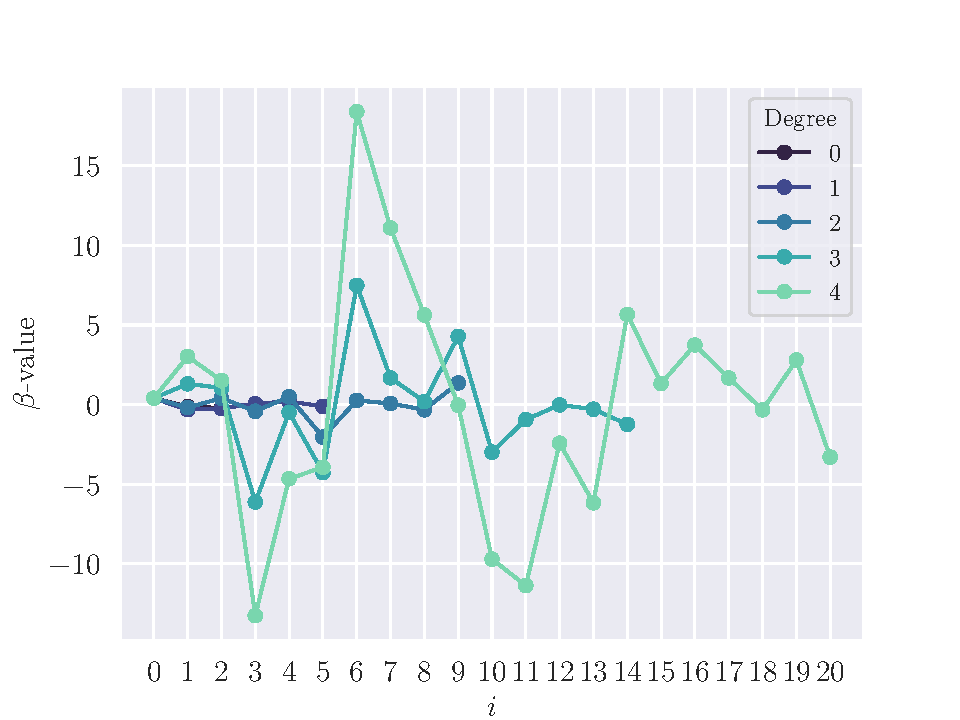
\includegraphics[width=0.9\linewidth]{project-1/latex/figures/ols_beta_smooth_scaled_N50.pdf}
    \caption{The figure shows $\beta$ values for the OLS model, with features of polynomial degree up to fifth order. The index $i$ denotes the index of $\beta_{i}$.The model was trained and tested on synthetic data without stochastic noise.}
    \label{fig:ols_beta_smooth}
\end{figure}
\begin{figure}
    \centering
    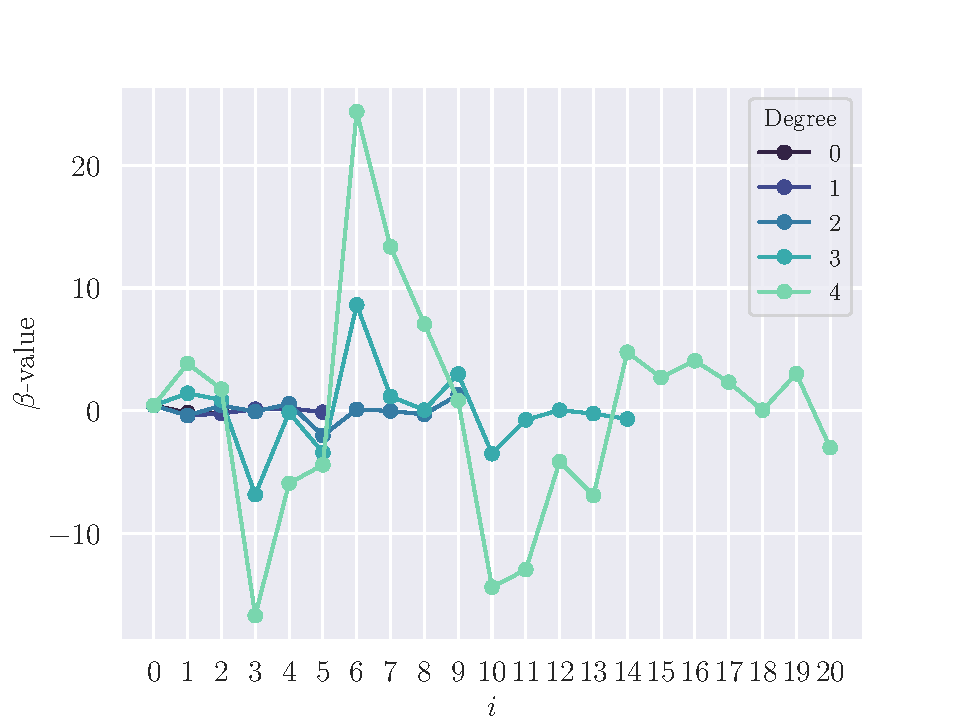
\includegraphics[width=0.9\linewidth]{project-1/latex/figures/ols_beta_scaled_N50.pdf}
    \caption{The figure shows $\beta$ values for the OLS model, with features of polynomial degree up to fifth order. The index $i$ denotes the index of $\beta_{i}$. The model was trained and tested on synthetic data which included stochastic noise $\mathcal{N}(0, 0.1)$.}
    \label{fig:ols_beta_smooth}
\end{figure}
\begin{figure}
    \centering
    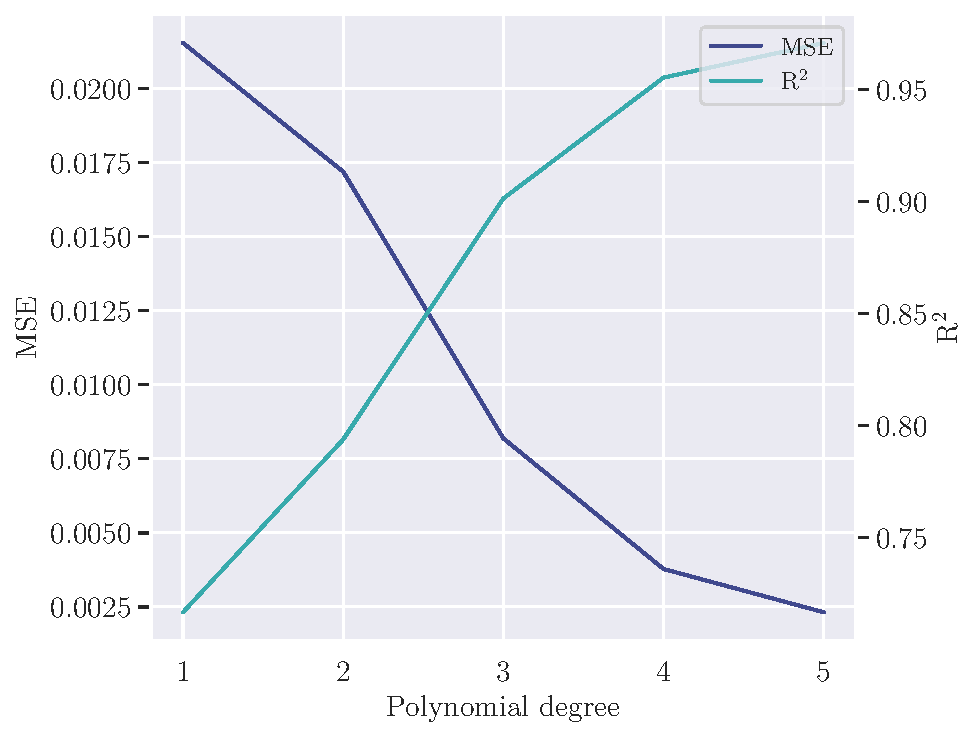
\includegraphics[width=0.9\linewidth]{project-1/latex/figures/ols_error_smooth_scaled_N50.pdf}
    \caption{MSE and R$^{2}$-score computed from predictions on test data, as a function of the polynomial degree of the input features. The model was trained and tested on synthetic data without stochastic noise.}
    \label{fig:ols_error_smooth}
\end{figure}
\begin{figure}
    \centering
    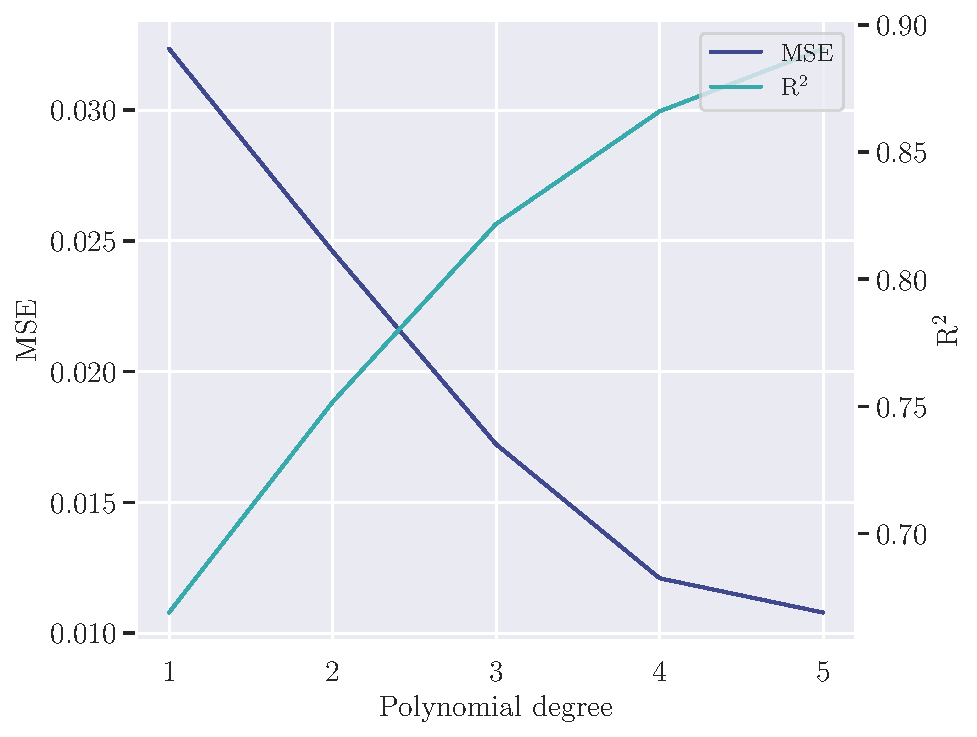
\includegraphics[width=0.9\linewidth]{project-1/latex/figures/ols_error_scaled_N50.pdf}
    \caption{MSE and R$^{2}$-score computed on test data, as a function of the polynomial degree of the input features. The model was trained and tested on synthetic data which included stochastic noise $\mathcal{N}(0, 0.1)$.}
    \label{fig:ols_error}
\end{figure}

I performed the Ridge regression for a large number of hyper-parameters, to determine a optimal range of values for $\lambda$. 
\begin{figure}
    \centering
    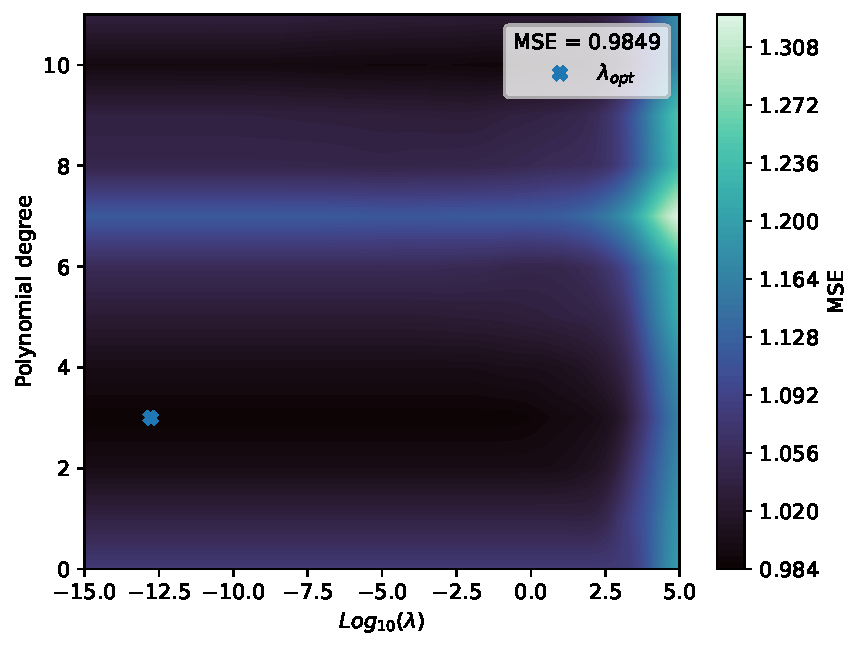
\includegraphics[width=0.9\linewidth]{project-1/latex/figures/dev-figs/lmbda_opt.pdf}
    \caption{The figure shows Ridge regression's MSE computed as a function of $\lambda$ and polynomial degree $P$, where the optimal value for $\lambda$ and $P$ is marked by an X.}
    \label{fig:lmbda_opt}
\end{figure}